%% Use the hmcposter class with the thesis document-class option.
\documentclass[thesis]{hmcposter}

\usepackage{mathtools}
\usepackage{amsmath}
\usepackage{libertinus}
\renewcommand\familydefault\sfdefault

\usepackage{enumitem}
\setlist[itemize]{
  left=1em..2em,
}

\usepackage{graphicx}
\usepackage{natbib}
\usepackage{booktabs}
\usepackage{subfig}
\usepackage{textcomp}
\usepackage{url}

\author{Kye Shi}
\posteryear{2022}
\title{Games for one, games for two!\\\LARGE\P{} vs \NP{} vs \SigmaP2 and more…}

\class{Math 197: Senior Thesis}

\advisor{Nicholas J. Pippenger}
\reader{Arthur Benjamin}

\usepackage{colortbl}
\setlength\arraycolsep{.5em}
\setlength\arrayrulewidth{2pt}
\arrayrulecolor{gray}

\usepackage{complexity}

\pagestyle{fancy}


\tikzset{
  input/.style={
    circle,
    fill,
    inner sep=0pt,
    minimum size=3pt,
  },
  gate/.style={
    draw,
    line width=2pt,
    rounded corners=1em/8,
  },
  pipe/.style={
    line width=2pt,
    rounded corners=1em/2,
    to path={
      (\tikztostart)
      -- ($ (\tikztostart -| \tikztotarget)!1/2!(\tikztostart) $)
      %-- ($ (\tikztotarget)!1em!(\tikztostart |- \tikztotarget) $)
      -- (\tikztotarget)
    },
    -Stealth,
  },
  over/.style={
    preaction={
      draw=white,
      line width=8pt,
      -,
    },
  },
  gates/.style={
    row sep=1em, column sep=3em, matrix of math nodes,
  },
  input/.style={
    circle,
    inner sep=0pt,
    minimum size=1em,
    fill,
    fill opacity=1/4,
    text opacity=1,
  },
  vertex/.append style={
    line width=2pt,
  },
}

\begin{document}


\begin{poster}

\section{Puzzles, games, and hierarchies}

\NP-complete problems

P vs NP problem.

what is NP?  useful way to understand it: puzzles, or games with a single turn.
a well-known example is the Sudoku puzzle


takes us farther: games with 2 turns fall into a class known as sigma2p, games
with k sigmakp (and yes, np=sigma1p).  together, these classes form the
polynomial hierarchy,



definition of a k-turn game.

\section{First stop: boolean circuits}

\Term{Boolean circuits} consist of \Term{wires}, which carry \True/\False{}
values, sent through various \Term{logic gates}:
\[
  \begin{array}{c|cl}
    \NOT & ¬x & \text{flips the value of \(x\)} \\
    \AND & x∧y & \text{\True{} iff both of \(x,y\) are \True} \\
    \OR & x∨y & \text{\True{} iff at least one of \(x,y\) are \True}
  \end{array}
\]

For example, the circuit below returns \True{} if and only if at least \(2/3\)
of its inputs are \True:

\begin{center}
  \begin{tikzpicture}
    \matrix[gates, ampersand replacement=\&]{
      |[input](x)|x \& |[gate](xy)|∧ \\
      |[input](y)|y \& |[gate](yz)|∧ \&\& |[gate](or')|∨ \\
      |[input](z)|z \& |[gate](zx)|∧ \\
    };

    \node[gate](or) at ($ (xy)!1/2!(or') $){\(∨\)};

    \draw[pipe] (y) to (xy.south west);
    \draw[pipe] (y) to (yz);
    \draw[pipe] (z) to (yz.south west);
    \draw[pipe] (z) to (zx);
    \draw[pipe, over] (x) to (zx.north west);
    \draw[pipe] (x) to (xy);

    \draw[pipe] (xy) to (or);
    \draw[pipe] (yz) to (or);
    \draw[pipe] (or) to (or');
    \draw[pipe] (zx) to (or');

    \draw[pipe] (or'.east) -- +(2em,0) node[right]{\(xy∨yz∨zx\)};

  \end{tikzpicture}
\end{center}

Here is a circuit that \emph{never} returns \True:

\begin{center}
  \begin{tikzpicture}
    \matrix[gates, ampersand replacement=\&]{
      \& |[gate](not)|¬ \& |[gate](and)|∧ \\
      |[input](x)|x \\
    };

    %\draw[pipe] (x) to (buf);
    \draw[pipe] (x) -- (not);
    \draw[pipe] (x) to (and);
    \draw[pipe] (not) to (and);

    \draw[pipe] (and) -- +(2em,0) node[right]{\(x∧¬x=\False\)};

  \end{tikzpicture}
\end{center}

\subsection{\Problem{Circuit Satisfiability} games are hard}

Some circuits are possible to \Term{satisfy}, i.e. cause to output \True; some
are not.  The game: \emph{given a circuit, can you satisfy it?}

NP-complete because circuits are universal; basic building blocks of logic \&
computers, pretty much any statement can be encoded using booleans.

k-turn games definition, also np-complete.

\section{Graph-coloring games}

Assign to each vertex in a graph one of three colors: \(\Colors\).  The coloring
is \Term{proper} if every two neighboring vertices have different colors:

\begin{center}
  \tikzset{
    pics/four/.style n args={4}{
      code={

        \coordinate[vertex, fill=ks#1](a) at (1em,0);
        \coordinate[vertex, fill=ks#2](b) at ($ (a) + (120:2em) $);
        \coordinate[vertex, fill=ks#3](c) at ($ (a) + (180:2em) $);
        \coordinate[vertex, fill=ks#4](d) at ($ (a) + (60:2em) $);

        \draw[line width=2pt] (a) -- (b) -- (c) -- (a) -- (d);

      },
    },
    common baseline/.style={text depth=1em/3, text height=2em/3},
  }
  \begin{tikzpicture}

    \matrix[column sep=4em] {
      \pic{four=2100}; & \pic{four=2120}; \\
      \node[common baseline]{proper}; & \node[common baseline]{improper}; \\
    };

  \end{tikzpicture}
\end{center}

Some graphs are impossible to properly 3-color:

\begin{center}
  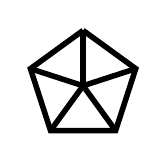
\begin{tikzpicture}
    \coordinate[vertex](o);
    \foreach \i in {0,...,4} {
      \coordinate[vertex](v\i) at ({360/5*\i+90}:2em);
      \draw[line width=2pt] (o) -- (v\i);
    }
    \draw[line width=2pt] (v0) -- (v1) -- (v2) -- (v3) -- (v4) -- (v0);
  \end{tikzpicture}
\end{center}

The game: \emph{given a graph, can you find a proper coloring for it?}

\subsection{Are graph-coloring games hard?}

Yes!  Convert from circuits to graphs as follows:

Assign so-and-so input vertices to which players; last player fills out
remaining colors on gate gadgets.

Requiring each player to play a proper move, constrains their colorings to be
consistent with boolean circuit outputs.

\section{Exact-cover games}

Menu, select items


\subsection{Are exact-cover games hard?}

Convert from circuits to graphs.

\section{Conclusions}

Rather than just a summary of your findings (which you presented in
the previous section), write your \emph{conclusions} based on those
results---what have you learned, and what does what you've learned
mean for your reader, the world at large, and your future research?

\section{For more information…}

\begin{itemize}[nosep]
  \item Feel free to email me at \url{kwshi@hmc.edu}.
  \item Check out the project website at \url{TODO}
  \item download the full thesis report at \url{insert claremont thesis URL here}
  \item GitHub page: \url{https://github.com/kwshi/hmc-math-thesis}
\end{itemize}

\bibliographystyle{hmcmath}
\bibliography{sampleposter}

\section{Acknowledgments}

If there are people or institutions that were particularly helpful
to you during your research, thank them here.  It's especially
important to mention anyone who gave you money.


\end{poster}

\end{document}
